\chapter{\IfLanguageName{dutch}{Stand van zaken}{State of the art}}
\label{ch:stand-van-zaken}

% Tip: Begin elk hoofdstuk met een paragraaf inleiding die beschrijft hoe
% dit hoofdstuk past binnen het geheel van de bachelorproef. Geef in het
% bijzonder aan wat de link is met het vorige en volgende hoofdstuk.

% Pas na deze inleidende paragraaf komt de eerste sectiehoofding.

\section{Inleiding}
Dit overzicht biedt inzicht in de huidige stand van zaken en vormt de basis voor een weloverwogen keuze bij de ontwikkeling van een Proof of Concept (PoC). Dit betreft zowel de technische als de juridische aspecten. Daarnaast wordt in dit deel ook stilgestaan bij het belang van een vlot supportproces binnen IT.

Concreet komen de volgende onderwerpen aan bod:
\begin{itemize}
    \item \textbf{IT-support chatbot} – Wat zijn de mogelijkheden van om een IT-support chatbot te maken aan de hand van een LLM en welke factoren moeten in overweging worden genomen?
    \item \textbf{De AI Act en de belangrijkste richtlijnen} – Een overzicht van de relevante wet- en regelgeving en de impact hiervan op RAG-toepassingen.
    \item \textbf{Best practices voor IT-supportprocessen} – Inzichten in hoe RAG kan worden toegepast binnen IT-support en welke methodologieën het best kunnen worden gevolgd.
\end{itemize}

De nadruk zal voornamelijk liggen op het eerste onderwerp, \textit{IT-support chatbot: wat zijn de mogelijkheden en welke factoren moeten in overweging worden genomen?}, aangezien dit een cruciale factor is voor het maken van een doordachte keuze bij de verdere uitwerking van de PoC. Indien nodig zullen de overige onderwerpen verder worden uitgediept.

\section{IT-support chatbot}

    \subsection{Introductie}
    
    Om een IT-support chatbot te maken zijn verschillende zaken die in overweging moeten worden genomen. Aan de hand van een LLM model zijn er twee grote opties die zich aandienen om dit te maken. Aan de ene kant kan gekozen worden voor Retrieval-Augmented Generation (RAG) aan de andere kant is er Cache-Augmented Generation (CAG). Zowel RAG als CAG maken gebruik van een LLM om aan de hand van eigen documenten de kennis die de LLM heeft te verhogen en te verbeteren. Echter hebben beide bepaalde voor- en nadelen en is het noodzakelijk om deze in rekening te brengen om een weloverwogen keuze te maken voor een PoC. 
    
    \subsection{Retrieval Augmented Generation}
    \subsubsection{Introductie}   
    \textit{Large Language Models} (LLM) hebben de afgelopen jaren een enorme opmars gemaakt en vandaag de dag hebben deze modellen een brede impact op verschillende domeinen in de samenleving. Ondanks hun indrukwekkende mogelijkheden brengen LLM’s ook enkele nadelen met zich mee. Zo kunnen ze hallucineren, beschikken ze niet altijd over de meest actuele informatie, en missen ze vaak diepgaande domeinspecifieke kennis.  
    
    Een mogelijke oplossing voor deze beperkingen is \textit{Retrieval-Augmented Generation} (RAG). Deze techniek combineert de kracht van LLM’s met externe databronnen om nauwkeurigere en beter onderbouwde antwoorden te genereren. In deze sectie wordt toegelicht wat RAG is, hoe het werkt en op welke manier het kan bijdragen aan de ontwikkeling van een effectieve support chatbot.
    
    \paragraph{Wat is RAG}
    RAG staat voor Retrieval-Augmented Generation en is, zoals eerder vermeld, een techniek die een antwoord biedt op de tekortkomingen van klassieke LLM’s. Door gebruik te maken van externe databronnen kunnen betere resultaten worden behaald dan met een traditionele LLM. Deze techniek maakt het mogelijk om domeinspecifieke data te integreren en de modellen bij te werken met actuele informatie. Hierdoor kunnen klassieke LLM’s verrijkt worden met nieuwe, up-to-date data die voldoet aan specifieke behoeften \autocite{Wu2024}.
    
    Om RAG in de praktijk toe te passen, moeten een aantal stappen worden doorlopen. Deze worden in het volgende deel nader toegelicht, maar samengevat bestaat het proces uit de volgende fasen:
    
    \begin{enumerate}
        \item \textbf{Ophalen}
        \item \textbf{Verrijking}
        \item \textbf{Generatie}
    \end{enumerate}
    
    Deze stappen worden in het volgende deel uitgebreid besproken. Aan het einde van dit proces kan een gebruiker de functionaliteiten van een LLM koppelen aan de relevante documenten en gegevens die benodigd zijn.
    
    \subsubsection{Hoe werkt RAG}
    
    De bedoeling van RAG is om een LLM te verrijken met specifieke kennis om de gebruiker te helpen bij het beantwoorden van specifieke vragen. Om dit tot stand te brengen moeten drie hoofdonderdelen aan bod komen. Het eerste onderdeel is het ophalen van relevante informatie (Retrieval). De tweede stap is verrijken van het antwoord op basis van de beschikbare documentatie. Ten slotte volgt de generatie, waarbij een LLM wordt gebruikt om een antwoord te formuleren op de gestelde vraag.
    
    Hieronder is een figuur te zien die dit proces illustreert.
    
    \begin{figure}[H]
        \centering
        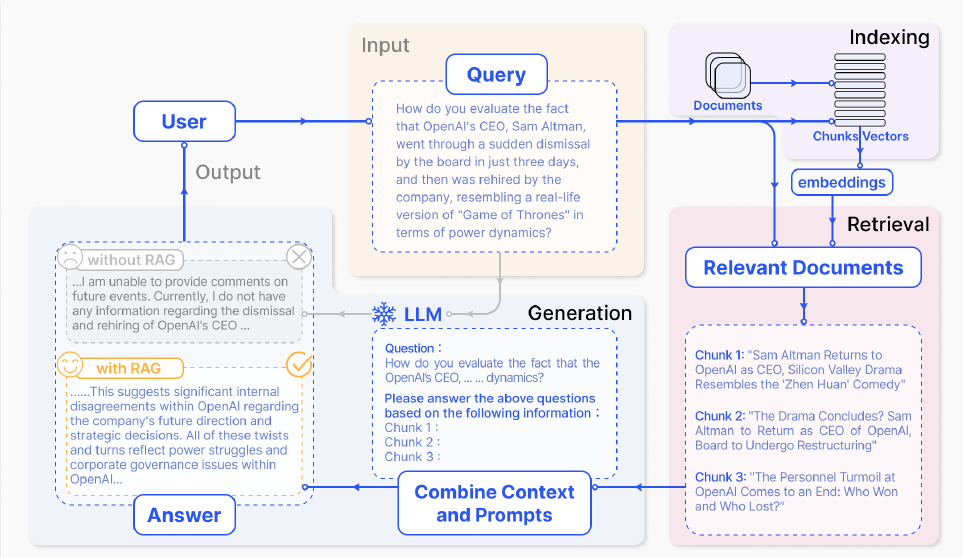
\includegraphics[width=\textwidth]{RagGao2023.png}
        \caption{Een generieke RAG architectuur \cite{Gao2023}}
        \label{fig:Rag process}
    \end{figure}
    
    \paragraph{Ophalen}
    
    %TODO verder uitschrijven en hier nog andere details over maken misschien opzoeken waar indexeren hier in komt in andere papaers zoals Goa2023 of Zhoa2024
    %TODO om hier te bespreken is het volgende een korte introductie, figuur veranderen naar die van Gao 2024 en dan starten met chunks en het voorbereiden van de LLM met de documenten die je wilt.
    
    %TODO laten corrigeren gramaticaal en de delen die hierin worden besproken verder uitbreiden met meer tekst zdat het langer is dan 2 zinnen.
    % gebruik figuur 2 van Wu2024 om te illustreren
    Vooraleer de LLM kan ondervraagt worden met informatie die we in de LLM steken door deze met de documenten te verrijken is eerst heel wat voorbereidend werk nodig. Het proces bestaat eruit om aan de hand van een vector database relevante documenten samen met de gestelde te gaan injecteren samen met de LLM om tot een goed antwoord te komen. Hiervoor moeten een aantal stappen ondernomen worden.
    
    Ten eerste moet een selectie gemaakt worden van de relevante documenten en worden opgedeeld in kleinere delen of zoals in de vakliteratuur wordt genoemd het verdelen van documenten in “chunks”. Dit wordt hoofdzakelijk gedaan omdat sommige documenten qua lengte te groot zijn om verder te kunnen op een effuiciëte manier te kunnen verwerkt worden. Daarnaast helpen chunks om precieze informatie in op te halen uit de vector database.  Om documenten in chunks te verdelen kunnen verschillende technieken worden toegapast te doen kunnen verschillende technieken worden toegepast. Er kan gewerkt worden op basis van een vast lengte of tokens. Dit zorgt ervoor dat elke chunk een gelijke lengte heeft. Een andere mogelijkheid is om, wanneer de documenten tekstdocumenten zijn, te werken met chunks op basis van een bepaalt aantal zinnen. Dit heeft als voordeel dat een chunk zijn semantiek beter kan behouden dan wanneer we werken met vaste lengte van chunks \autocite{Wang2024}.
    
    Dit met het uiteindelijke doel om deze chunks te vertalen naar embeddings die je in een vector database kan steken. Een embedding is de vector representatie van een tekstuele chunk. 
    
    Aangezien het RAG proces bestaat uit het toevoegen van documentatie om een bestaande LLM accurater of bepaalde kennis te geven is het niet zo dat voor iedere vraag die wordt gesteld aan de LLM we nood hebben om gebruik te maken van deze documentatie. Enkel wanneer een vraag gesteld wordt die een LLM niet kan behandelen moet gebruik gemaakt worden van RAG. Bijgevolg is het noodzakelijk om een classificatie te maken tussen query's waarbij het ophaling via RAG noodzakelijk is en waar niet \autocite{Wang2024}.
    
    Naast de classificatie is ook moet de informatie die aan het LLM model wordt gegeven worden opgedeeld in “chuncks” dit komt neer op het opdelen van documenten in kleinere delen op basis van bepaalde zaken. 
    \paragraph{Verrijken}
    \paragraph{Generatie}
        
    
    
    
    \subsection{Cache-Augmented Generation}
    \subsubsection{Introductie}
    
    \subsection{Retrieval Augmented Generation vs Cache-Augmented Generation}
    
    
    \subsection{LLM-modellen}
    Welke bestaande LLM-modellen kunnen worden gebruikt voor het ontwikkelen van een Retrieval-Augmented Generation (RAG)? 
    
    %TODO opzoeken wat LLM benchmarks zijn en hoe je ze in deze context kan gebruiken
    
    \paragraph{Introductie}
    Om te bepalen welke modellen het meest geschikt zijn voor de ontwikkeling van een RAG-model, is een objectieve meetmethode noodzakelijk. Gelukkig bestaan er verschillende platforms die LLM's vergelijken en rangschikken op basis van prestaties. In deze sectie bespreken we enkele van deze platforms en maken we een selectie van modellen die het meest geschikt lijken voor het bouwen van een RAG-model.
    
    %TODO overall dieper ingaan hoe ze te werk gaan als het gaat om vergelijken van een LLM dus de paper lezen en samenvatten wat je ermee kan gaan doen
    
    \paragraph{LiveBench} 
    Een platform dat LLM-modellen evalueert, is LiveBench. Dit platform stelt een rangschikking op voor verschillende modellen en biedt een actuele leaderboard die elke zes maanden wordt bijgewerkt. Voor deze bachelorproef zal gebruik worden gemaakt van de ranking afkomstig uit november 2024.
    
    LiveBench beoordeelt LLM-modellen op basis van zes categorieën. Binnen elke categorie worden meerdere taken uitgevoerd om een nauwkeurige beoordeling te verkrijgen. De zes categorieën zijn:
    \begin{itemize}
        \item Wiskundige vaardigheden (Math)
        \item Programmeervaardigheden (Coding)
        \item Redeneren en probleemoplossing (Reasoning)
        \item Data-analyse (Data Analysis)
        \item Volgen van instructies (Instruction Following)
        \item Begrip van natuurlijke taal (Language Comprehension)
    \end{itemize}
    
    Elke categorie wordt geëvalueerd op basis van specifieke taken. Dit resulteert uiteindelijk in een algemene rangschikking, waarin zowel de beste modellen per categorie als het beste presterende model overall worden geïdentificeerd.
    
    \begin{figure}[H]
        \centering
        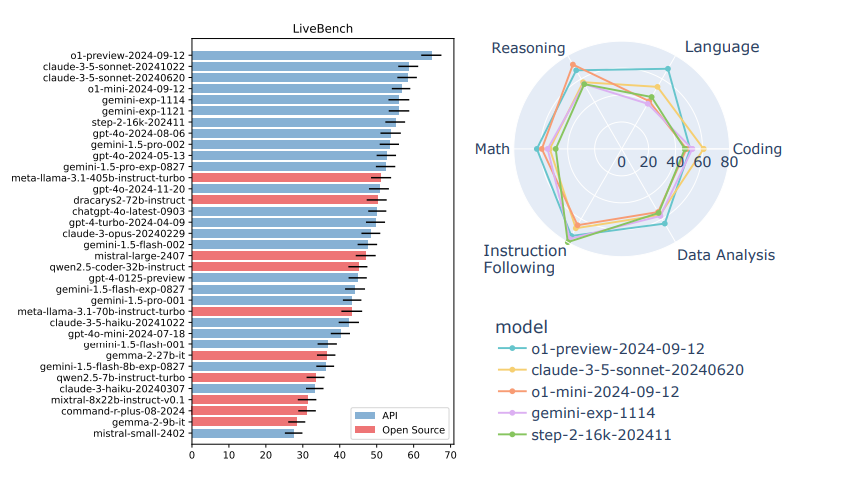
\includegraphics[width=\textwidth]{LiveBenchRanking.png}
        \caption{LiveBench ranking van verschillende LLMs.}
        \label{fig:livebench}
    \end{figure}
    
    \noindent\textbf{Bron:} \textit{LiveBench AI} \url{https://livebench.ai/#/details} (Geraadpleegd op 16 februari 2025).
    
    Uit de ranking van LiveBench kan geconcludeerd worden dat 3 verschillende organisaties elk een model aanbieden die vanuit globaal oogpunt tot de top 3 behoort. Deze top 3 zijn: 
    \begin{enumerate}
        \item claude-3-5-sonnet-20240620 van Anthropic
        \item Meta-llama-3.1-405b-instruct-turbo van Meta
        \item gpt-4o-2024-05-13 van OpenAI
    \end{enumerate}
    
    \subsubsection{Chatbot arena} 
    
    %TODO uitleggen hoe de scoring werkt van chatbot en eventueel uitleggen wat de verschillen zijn met LiveBench, ik denk vooral dat Chatbot arena getest wordt door mensen en zij hun mening op een grote schaal uitdrukken
    Een andere benchmark tool Chatbot arena, net zoals livebench is Chatbot arena een site die een actuele weergave biedt van de beste LLM's op basis van vooraf gedefinieerde catgeoriën. Op het moment van het schrijven van deze literatuurstudie is de top 3 LLM's volgens deze site de volgende:
    
    \begin{enumerate}
        \item GPT-4-Turbo van OpenAI
        \item GPT-4-0613 van OpenAI
        \item Mistral-Medium Mistral AI
    \end{enumerate}
    
    Hoewel het doel van beide benchmarks hetzelfde is is de manier van werken wel anders. ChatbotArena gaat gebruikers twee anonieme LLM modellen tegenover elkaar plaatsen, de gebruiker kan vervolgens een eigen vraag stellen en de gebruiker bepaalt zelf welke van de 2 het beste resultaat heeft opgeleverd.
    
    Het voordeel van deze methode is dat de LLM-modellen realistische cases moeten behandelen die door gebruikers zelf worden gesteld. Op basis van resultaten die de LLM modellen tonen kan een gebruiker zijn voorkeur meegeven. Het nadeel van deze manier van werken is dat de gebruikers die deze testen uitvoeren niet respresentatief zijn voor alle gebruikers van LLM-modellen. De gebruikers die deze testen uitvoeren zijn vaak mensen met een interesse in LLM-modellen of mensen die onderzoek doen in dit vakgebied. Desoondanks kan op basis van deze stemmen verscheidene modellen tegenover elkaar worden geplaatst. In januari 2024 werden ruim 240.000 stemmen uitgebracht door ongeveer 90.000 gebruikers \autocite{Chiang2024}. 
    
    %TODO zet hier ook de actuele ranking van beide benchmarks. Al was het maar om te duiden dat het een sterk veranderende wereld is waar en dat naar alle waarschijnlijkheid de modellen die nu worden gebruikt waarschijnlijk al achterhaald zullen zijn.
    
    \paragraph{Conclusie}
    Op basis van de 2 benchmarks die hier werden besproken kan niet meteen éénduidig besloten worden welke modellen het best zouden gebruikt worden voor het maken van het RAG model. Aangezien dit een zeer volatiele omgeving is met veel en snelle ontwikkelingen zijn de modellen die vandaag het beste scoren over een maand potentieel voorbij gestoken door nieuwe modellen. Desalniettemin bevatten deze benchmarks heel wat nuttige informatie en inzichten over de sterktes van bepaalde modellen tegenover andere modellen. 
    

\section{De AI Act en de belangrijkste richtlijnen}
Wat houdt de AI Act in, en wat zijn de belangrijkste richtlijnen die hierin moeten worden gevolgd?

\section{Best practices voor IT-supportprocessen}
Wat zijn de bestaande best practices voor de organisatie van IT-supportprocessen?
